\documentclass{article}

\usepackage[a4paper]{geometry}
\usepackage[ngerman]{babel}
\usepackage[utf8]{inputenc}
\usepackage[T1]{fontenc}
\usepackage{hyperref}
\usepackage{graphicx}

\graphicspath{ {./images/} }

\hypersetup{
    colorlinks=true,
    linkcolor=black,
    filecolor=black,      
    urlcolor=black,
}

\begin{document}

\begin{titlepage}
	\begin{flushleft}
		TH Brandenburg \\
		Online Studiengang Medieninformatik \\
		Fachbereich Informatik \\
		Softwaretechnik \\
		Prof. Dr-Ing. Martin Schafföner
	\end{flushleft}

	\vfill

	\begin{center}
		\Large{Einsendeaufgabe 1: Requirements Engineering}\\[0.5em]
		\large{Sommersemester 2021}\\[0.25em]
		\large{Abgabetermin 18.04.2021}
	\end{center}

	\vfill

	\begin{flushright}
		Maximilian Schulke \\
		Matrikel-Nr. 20215853
	\end{flushright}
\end{titlepage}

\tableofcontents

\newpage

\section{Aufgabenstellung}


\vspace{100px}
\begin{center}
	\large{To be inserted!}
\end{center}
\vspace{100px}

\section{Projekt}

Als Projekt für dieses Semester verwende ich eine Idee, die mir schon seit längerem im Kopf rumgeistert
– einen kleinen, minimalistischen \emph{Tiling Window Manager} für Linux bzw. X11, der deutlich flexibler
und entwicklerfreundlicher ist als bestehende, vergleichbare Software.

\subsection{Zusammenfassung der Domain}

Für den Fall, dass Sie noch keinen Kontakt mit dieser Domain hatten, gehe ich im folgenden kurz darauf ein,
welche Aufgaben ein \emph{Tiling Window Manager} (kurz. \emph{TWM} oder nur \emph{WM}) typischer Weise
übernimmt. Die generelle Aufgabe eines WM's besteht hauptsächlich darin sich um die Kommunikation mit dem
\emph{Window-Server} (i.d.R. X11 oder Wayland auf Linux, Quartz Compositor auf MacOS) zu kümmern, und die
tatsächliche Anordnung der Fenster auf dem Bildschirm zu regeln (in Ebenen, Kacheln etc. – die Möglichkeiten
sind nahe zu unbegrenzt). Typische \emph{Window Manager} von z.B. MacOS können diverse, für uns als Endnutzer
mittlerweile als üblich angesehene, Anordnungen wie Floating, Split-Screen und Fullscreen realisieren. \par
Ein \emph{Tiling Window Managers} hat nun die Besonderheit, dass er anders als von Windows, MacOS oder diversen
Linux Desktop-Umgebungen bekannt, die Aufteilung der Fenster automatisch und bestmöglich regelt. Typischerweise
hat ein \emph{TWM} eine feste Konfiguration mit Layouts, in die er die Fenster einsortieren kann (z.B. ``Master
and Stack``). Somit muss sich der Anwender eines solchen \emph{TWM's} (zumindest initial) nicht selber um die
Anordnung seiner Fenster kümmern. Desweiteren zählt die Möglichkeit, Keybindings zur Navigation oder Veränderung
der Aufteilung zu definieren, zu den typischen Features eines \emph{Tiling Window Managers}.

\subsection{Projekt-Ziel}

Das Problem von bestehenden \emph{Window Managern} ist in der Regel deren Alter (bspw. ist das Projekt ``Toms
Window Manager`` im Jahr 1987 entstanden). Aufgrund des Alters sind viele dieser \emph{Window Manager} noch in
C, C++ oder einer vergleichbaren Sprache verfasst worden und mit der Zeit immer weiter gewachsen. Dies macht es
deutlich schwerer als es sein müsste, grundlegende Änderungen, die nicht von den Entwicklern vorhergesehen waren,
vorzunehmen. \par
Ziel ist es einen \emph{minimalen Window Manager} zu entwickeln, der \emph{durch eigenen Programm-Code konfiguriert}
und erweitert werden kann. Dieses Konzept ist schon öfter Implementiert worden (als Inspiration für dieses Modell
dienen die Projekte \emph{XMonad\footnotemark} und \emph{DWM\footnotemark}), allerdings sind diese Projekte leider
meistens schlecht dokumentiert und haben i.d.R. unnötig komplexe \emph{API's}. Zu den typischen Anwendern dieser
\emph{Window Manager} gehören Entwickler und Power User.

\footnotetext[1]{wurde 2007 erstmals veröffentlicht. Wurde in Haskell geschrieben und wird auch damit
	konfiguriert. Siehe \url{https://xmonad.org/} für weitere Informationen.}
\footnotetext[2]{ist ein äußerst kleiner (unter 2000 Zeilen Source-Code) Window Manager geschrieben in C. Er
	hat keine Konfigurationsdatei und wird durch Patchen des Codes konfiguriert. Siehe \url{https://dwm.suckless.org/}
	für weitere Informationen.}

\section{Erfassung der Anforderungen}

Zur Erfassung der Anforderungen verwende ich das Projektmanagement Feature von GitHub. Dieses hat zumindest im
kleinen Rahmen diverse Vorteile gegenüber herkömmlicher Software für Agile Projekte (z.B. Jira von Atlassian).
Unter anderem Folgende:

\begin{itemize}
	\item Übersichtlicher durch kleineren Umfang und somit leichter zu Bedienen
	\item Direkte Integration mit dem Entwicklungsprozess (Issues können z.B.
	      geschlossen werden sobald ein Feature gemerged wurde)
	\item Nutzer der Software können direkt Issues anlegen
\end{itemize}

Diese Entscheidung hat keine Endgültigkeit. Wenn es ein echtes Team mit einem klaren Vorgehensmodell gibt, können
andere Tools besser geeignet sein. Außerdem sei erwähnt, dass Jira mit diversen Integrationen erweitert werden
kann, um die oben beschriebene Funktionalität nachzurüsten. Zur geordneten Erfassung von Anforderungen, deren
Priorisierung, Kategorisierung und Abnahme, reicht \emph{GitHub Projects} allerdings vorerst vollkommen aus. Es
gibt die Möglichkeit Sprint oder Kanban Boards anzulegen, diese zu automatisieren oder komplett eigene Prozesse
zu integrieren.

\vspace{0.5em}

\begin{figure}[h]
	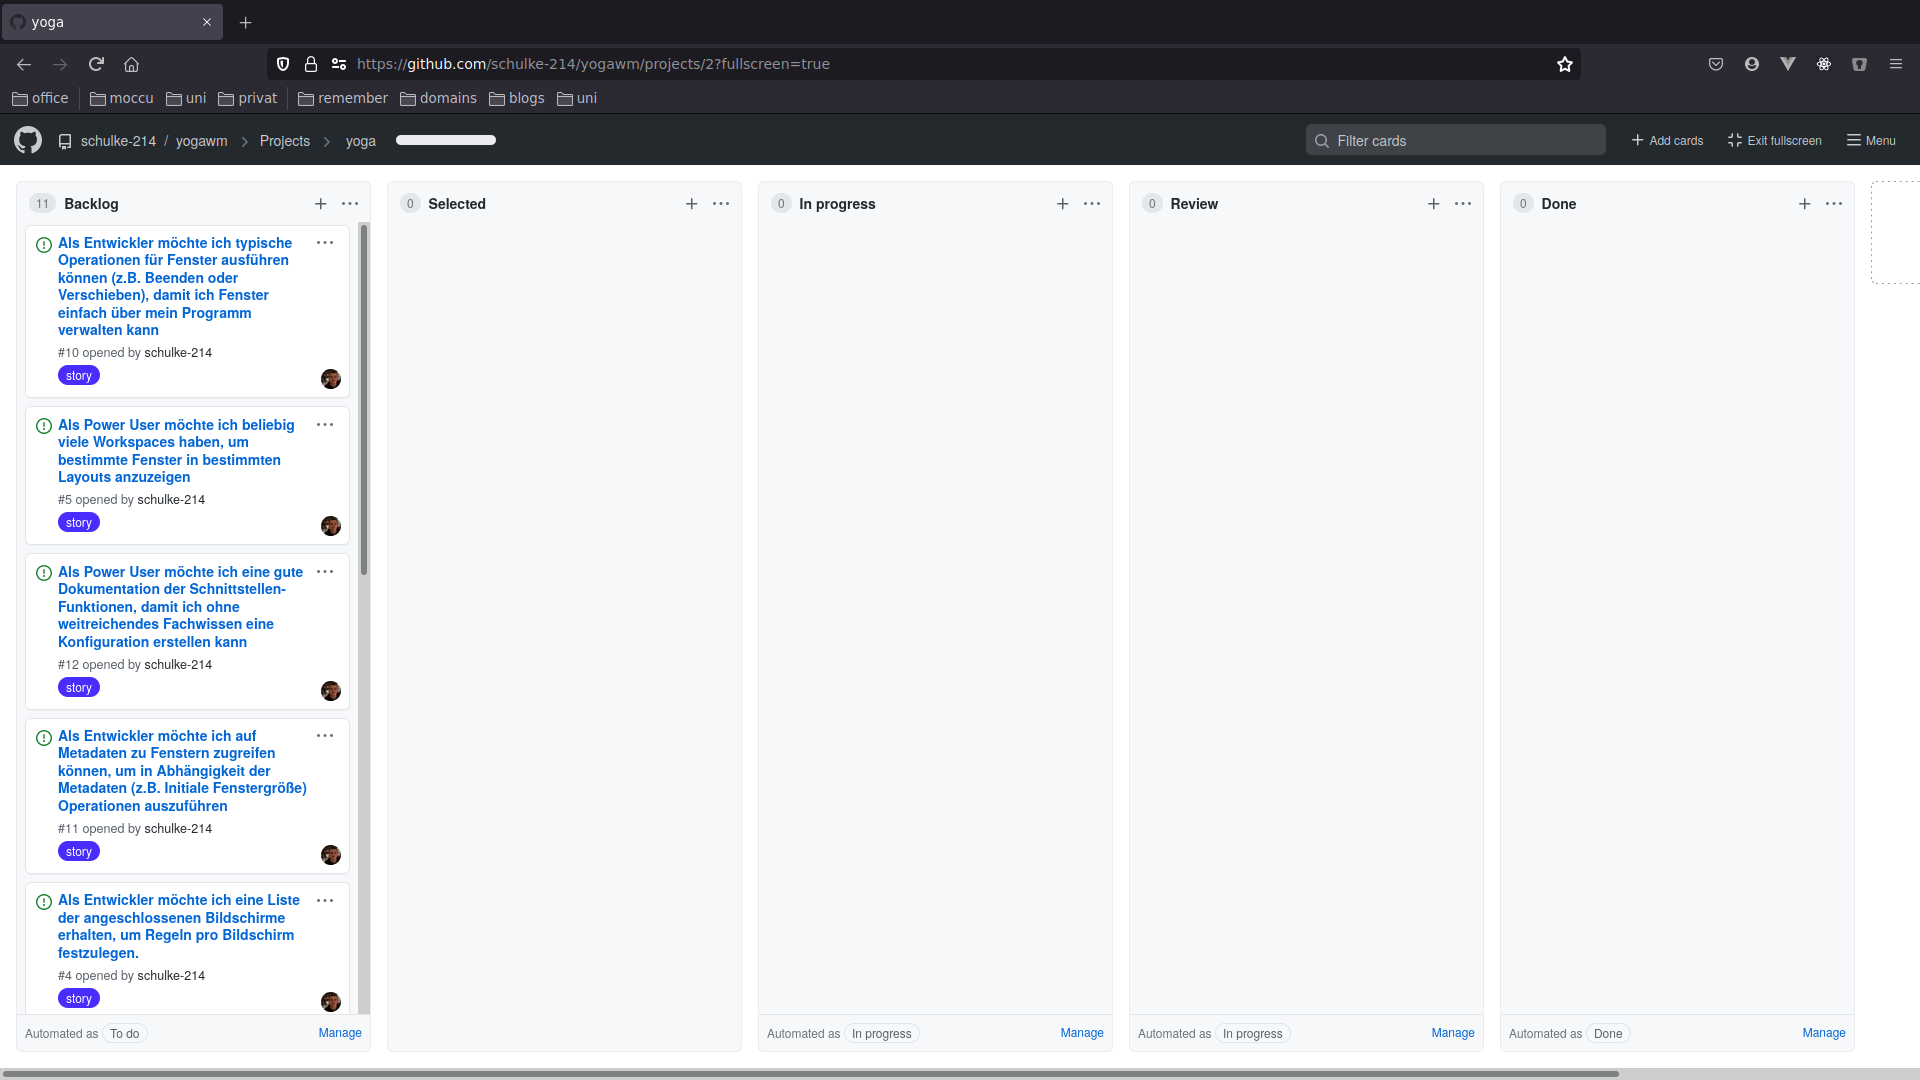
\includegraphics[width=0.6\textwidth]{github-projects}
	\centering
	\caption{\emph{GitHub Projects} Board}
\end{figure}

\newpage

\section{Anforderungen}


\end{document}